\chapter{Context}\label{chap:context}

\begin{sectionIntro}
    TODO
\end{sectionIntro}

\section{Company}

\subsection{CELAD}
One of its biggest clients in the embedded sector in Toulouse is Intel.
TODO

\subsection{Intel}
%TODO: ask AP if he is ok with this reuse
Intel is a big company, with multiple divisions.

Some key figures of Intel:
\begin{itemize}
\item Leading manufacturer of computer, networking and communications
  products,
  \item 300 Facilities in 50 countries,
  \item Over \$35B in Annual Revenues from customers in over 120
    countries,
\item 23 Consecutive years of positive net income,
\item Approximately 80,000 employees,
\item 43,000 technical degrees, 12,000 Masters in Science, 4,000
  PhD’s, 4,000 MBA’s,
  \item One of the top ten most valuable brands in the world for 10
    consecutive years,
\item Invests \$100 Million each year in education across more than 50
  countries,
  \item The single-largest voluntary purchaser of green power in the
    United States,
\item One of the top ten Linux \gls{kernel} contributors.
\end{itemize}

\subsection{Audio feature team in Toulouse}
The team I worked with is the audio feature team, in Toulouse.
They are responsible for the Audio \gls{hal} and the interface between the
librairies and the Android \gls{kernel}.


\section{Android}
During my internship, I worked on the \gls{android} platform.
Let's have an overview of the \gls{android} architecture to understand where
the Audio \gls{hal} is placed within this platform.

\subsection{Global Android architecture}

On the figure \ref{fig:archi}, the we can see the Audio \gls{hal} between the
Linux \gls{kernel} and the libraries layers.
\begin{figureGraphics}{Global Android architecture}{fig:archi}
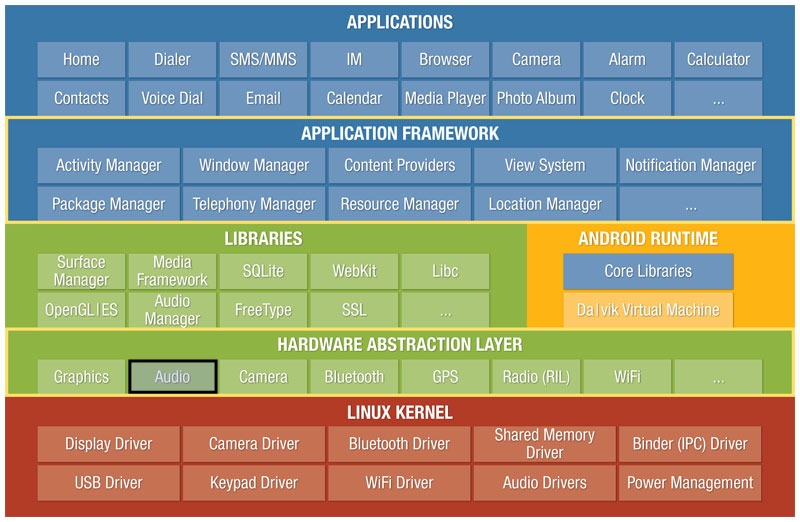
\includegraphics[width=\textwidth]{./src/img/android-archi-audio-hal.jpeg}
\end{figureGraphics}

\subsection{Intel Audio HAL}
Intel's Audio \gls{hal} for Android platforms is based around a generic, plugin-based solution: the \gls{pfw}.
It runs in the \emph{userland}, which is easier to maintain than kernel-space code.
Since this solution is plugin-based, it is easy to extend to add more subsystems if needed.

\begin{figureGraphics}{Intel Audio HAL}{fig:hal}
%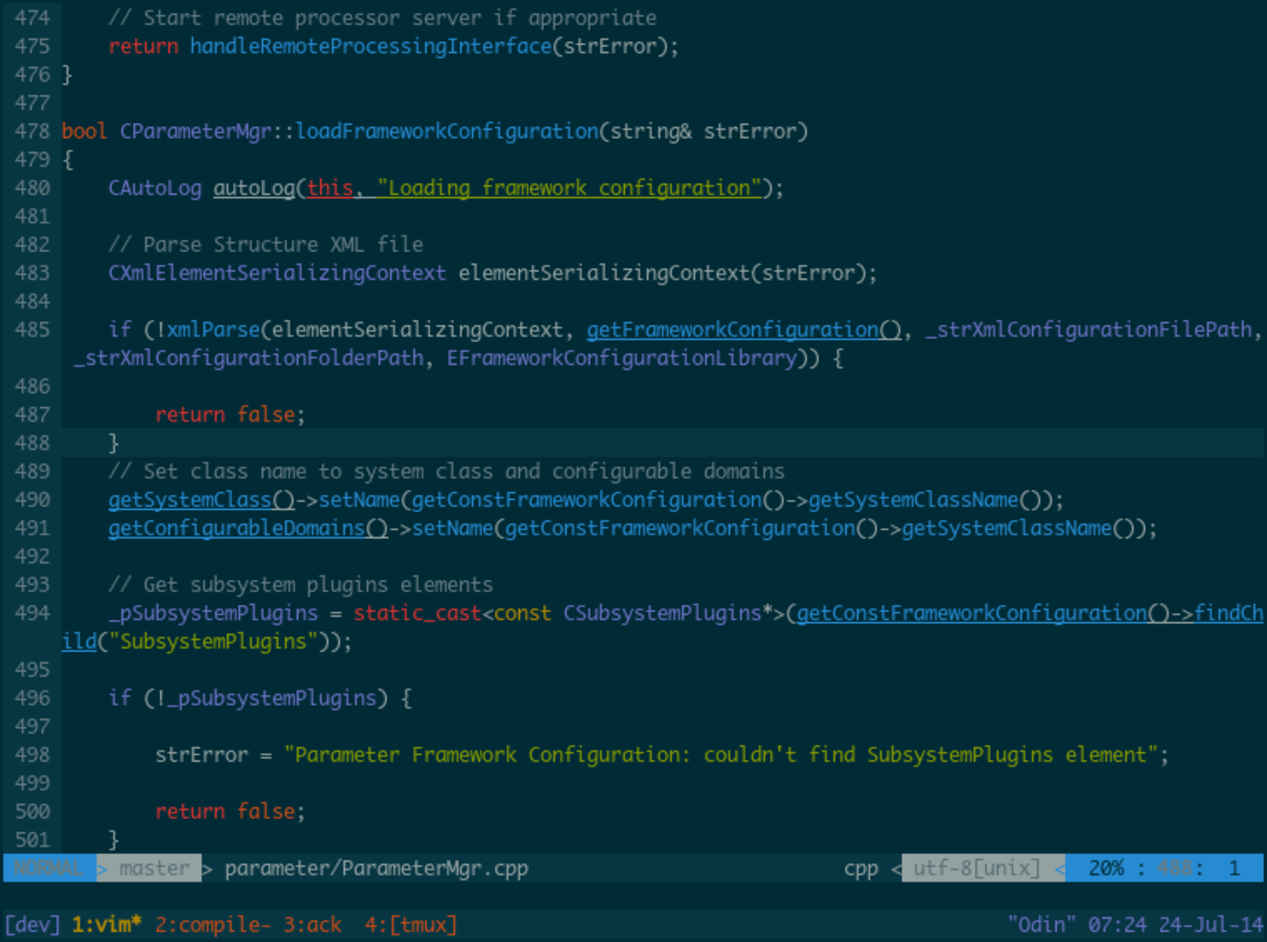
\includegraphics[width=\textwidth]{./src/img/setup.pdf}
    TODO Sylvain NDA?
\end{figureGraphics}

HAL, multiple platforms with different architectures.
Scalable, fully configurable, userland.
Tinyalsa
TODO

\subsection{Parameter-framework}
\label{sec:parameter-framework}
The Linux \gls{kernel} has a set of standard APIs, but the middleware layers do not have such standardization.

There is gap

No standards in middleware:
Big gap to fill


Middleware, gap, no standard.

\subsection{Topic of my internship}

I worked within the Intel Audio development team, as an \emph{agile
software developer}. The team is customers oriented, using \gls{scrum}
methodology (see chapter \ref{chap:organisation}). My tasks
within the team were focused around opensourcing the \gls{pfw} on
GitHub\footnote{\url{www.github.com/01org/parameter-framework}} to give it some
visibilty.


\section{Workflow and environment}
In this section, we will cover my daily workflow. This helps
to understand how I proceeded during my whole internship.

\begin{figureGraphics}{Developer workflow}{fig:workflow}
%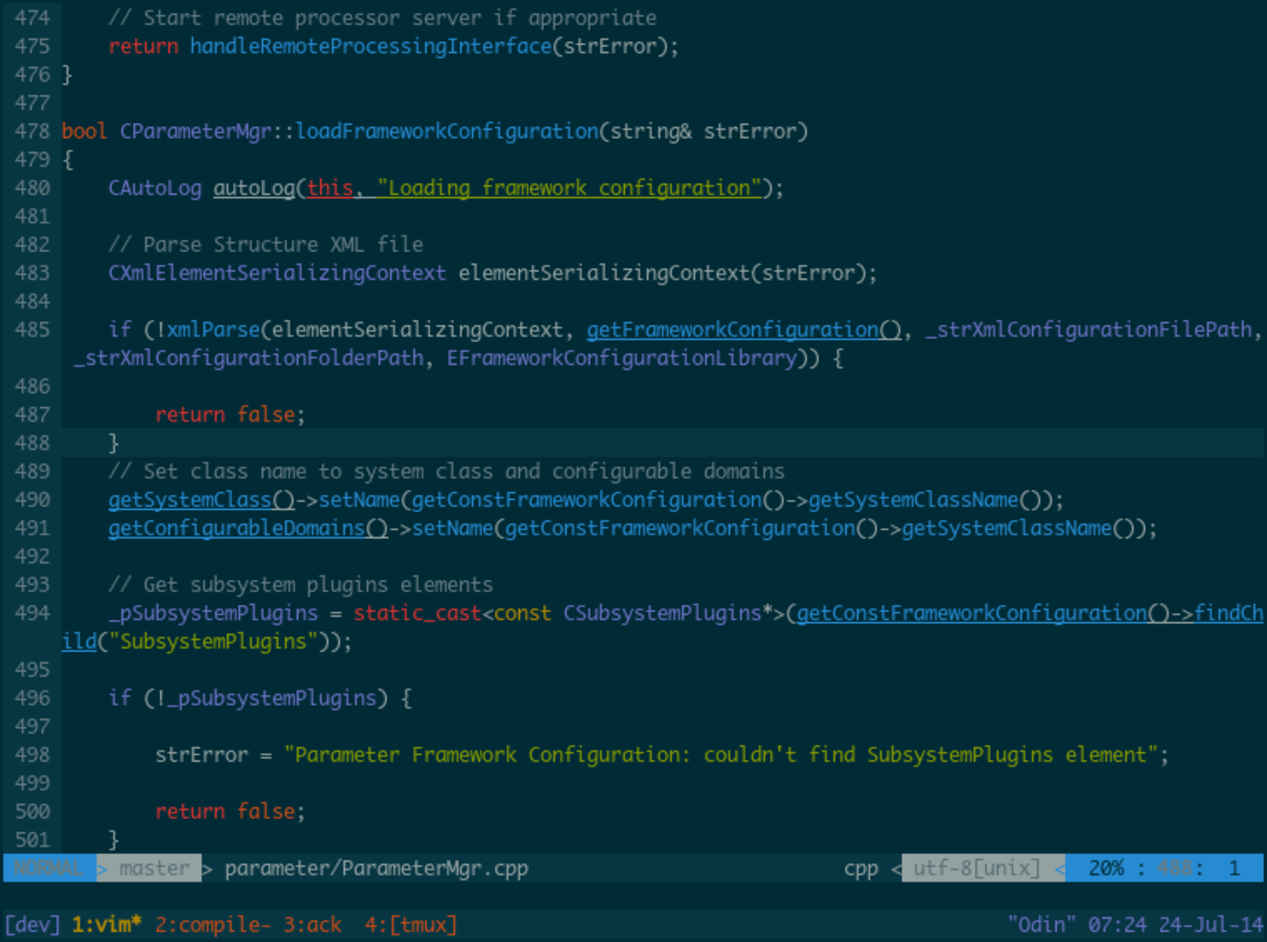
\includegraphics[width=\textwidth]{./src/img/setup.pdf}
    TODO
%Development => review => rework => review => submission to integration team
\end{figureGraphics}


\subsection{Development}
Since compiling the Android source tree requires a lot of computing power,
most of developers of our team are working remotely, via ssh.
The server we are connecting to is far more powerful than the desktops we use.
With it 32 cores and it's 2 TeraBytes of SSD, compilation time was far less time-consuming
than compiling locally!

I also worked on that server. This constraints to use command line programs only.
During my internship, I sharpened my skills in \gls{vim} and discovered \gls{tmux}.
On the figure \ref{fig:setup} below, there is a screenshot of my development setup at Intel.

\begin{figureGraphics}{Development setup with vim and tmux}{fig:setup}
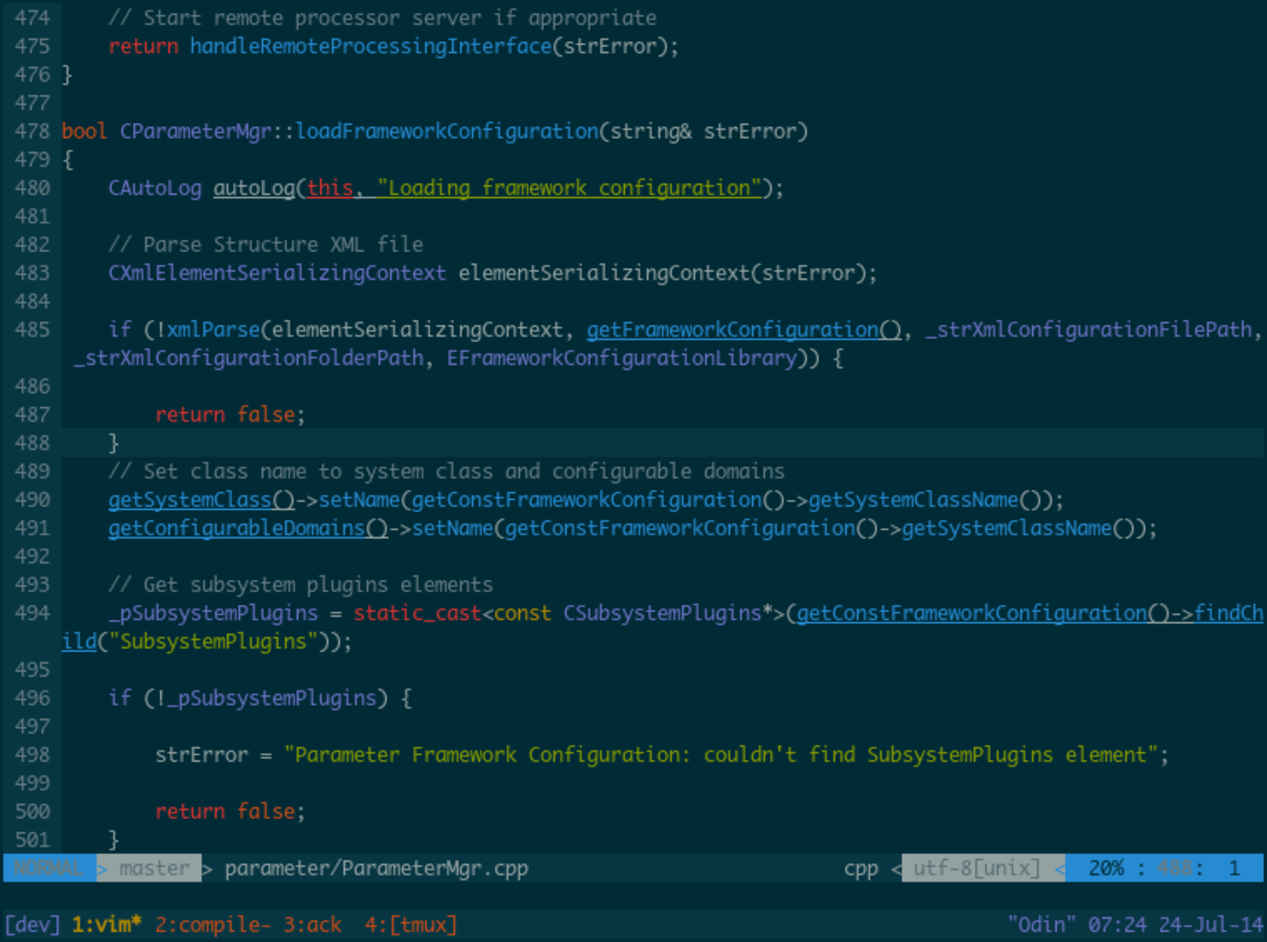
\includegraphics[width=\textwidth]{./src/img/setup.pdf}
\end{figureGraphics}

When the code is ready, I pushed it via \gls{git} on \gls{gerrit} to be reviewed.

\subsection{Code review}
Code quality matters. Clean code eases maintenance and is less error-prone.
Those facts are driving the team that I integrated at Intel. Naturally, all the
patches I have delivered during my internship have been reviewed and meet the
expected quality.

I have done some code review myself during this internship. It helps a lot to
understand how other people work. Viewing other peoples code also makes me come
up with new ideas to improve my own work.

\subsection{Submission to integration team}

